\chapter{Ciclos biogeoquímicos}\label{ch:b2:biogeochemical-cycles}

En marzo de 1958, un joven químico llamado Charles Keeling puso en marcha
un analizador de gases por infrarrojos en la ladera norte del Mauna Loa,
en Hawái, a tres kilómetros y medio por encima del Pacífico, donde el aire
está tan bien mezclado como puede estarlo. Esperaba medir una constante;
al cabo de un año tenía unos dientes de sierra --- el dióxido de carbono
subía cada invierno y bajaba cada verano a medida que los bosques del
hemisferio norte espiraban e inspiraban --- y, al cabo de unos pocos años,
una pendiente bajo los dientes de sierra que no se ha detenido desde
entonces. La \omterm{prop:b2:biogeochemical-cycles:carbon}{curva de Keeling} es la respiración de la biosfera vista desde
fuera, con una gráfica de fiebre dibujada encima. Este capítulo trata de
los ciclos que registra la curva: dónde se almacenan el carbono, el
nitrógeno, el fósforo y el azufre de los seres vivos, con qué rapidez se
desplazan entre \omterm{def:b2:biogeochemical-cycles:reservoir}{reservorios}, qué fija esas velocidades --- en su mayoría,
los metabolismos del \cref{ch:b2:microbial-metabolism} --- y qué ha hecho
una sola especie con cada ciclo en doscientos años.

\section{Reservorios, flujos y tiempos de residencia}

\begin{definition}[Reservorio, flujo, tiempo de residencia]\label{def:b2:biogeochemical-cycles:reservoir}
\index{reservorio}\index{flujo}\index{tiempo de residencia}\index{estado estacionario}\index{ciclo biogeoquímico}
Un \emph{ciclo biogeoquímico} es el movimiento de un elemento entre
\emph{reservorios} (la atmósfera, el océano, los suelos, la biomasa viva,
las rocas) mediante \emph{flujos} medidos en masa por año. Un reservorio
de masa $M$ con una salida total $F$ tiene un \emph{tiempo de
residencia} $\tau = M/F$, el tiempo medio que pasa un átomo en él; en
\emph{estado estacionario}, la entrada es igual a la salida y $M$ es
constante. Los ciclos están acoplados a través de la estequiometría de la
vida --- el \emph{cociente de Redfield} del plancton marino,
$\mathrm{C:N:P} =
106:16:1$ en átomos ---, de modo que el aporte del elemento más escaso
fija la velocidad a la que se absorben todos los demás.
\end{definition}

\begin{theorem}[El modelo de una caja]\label{thm:b2:biogeochemical-cycles:box}
\index{modelo de caja}\index{tiempo de relajación}
Si un \omterm{def:b2:biogeochemical-cycles:reservoir}{reservorio} pierde su contenido a una velocidad proporcional a lo que
contiene, $F_{\text{sal}} = M/\tau$, y recibe una entrada constante
$F_{\text{ent}}$, entonces
\[
\frac{\mathrm{d}M}{\mathrm{d}t} = F_{\text{ent}} - \frac{M}{\tau},
\qquad
M(t) = M^{*} + (M_0 - M^{*})\,e^{-t/\tau}, \qquad M^{*} = F_{\text{ent}}\tau :
\]
el \omterm{def:b2:biogeochemical-cycles:reservoir}{reservorio} se relaja hacia un \omterm{def:b2:biogeochemical-cycles:reservoir}{estado estacionario} proporcional a su
entrada, con el \omterm{def:b2:biogeochemical-cycles:reservoir}{tiempo de residencia} como constante de tiempo. Un aumento
brusco de la entrada eleva el \omterm{def:b2:biogeochemical-cycles:reservoir}{estado estacionario} en la misma proporción,
y el \omterm{def:b2:biogeochemical-cycles:reservoir}{reservorio} lo sigue en unos pocos $\tau$: un compartimento con un
\omterm{def:b2:biogeochemical-cycles:reservoir}{tiempo de residencia} de días (el amoníaco atmosférico, el nitrato de un
lago en primavera) sigue a sus fuentes; uno con un \omterm{def:b2:biogeochemical-cycles:reservoir}{tiempo de residencia} de
siglos (el carbono del océano profundo, la materia orgánica del suelo) las
integra, y la perturbación de un compartimento lento sobrevive a la
perturbación que la causó.
\end{theorem}
\begin{proof}
La ecuación es lineal con coeficientes constantes: el \omterm{def:b2:biogeochemical-cycles:reservoir}{estado estacionario}
$M^{*}$ anula el segundo miembro, y la desviación $m = M - M^{*}$
cumple $\dot m = -m/\tau$, de modo que $m = m_0 e^{-t/\tau}$. Si un
\omterm{def:b2:biogeochemical-cycles:reservoir}{reservorio} tiene varias salidas, $\tau$ lo fija su suma, $1/\tau = \sum_i
1/\tau_i$: domina el sumidero más rápido.
\end{proof}

\section{El ciclo del carbono}

\begin{proposition}[El balance del carbono]\label{prop:b2:biogeochemical-cycles:carbon}
\index{ciclo del carbono}\index{fracción atmosférica}\index{sumidero de carbono}\index{curva de Keeling}
En gigatoneladas de carbono (\unit{GtC}, $10^{12}$~kg), los principales
\omterm{def:b2:biogeochemical-cycles:reservoir}{reservorios} son la atmósfera (unas 880 en la década de 2020, 590 antes de
la industria), las plantas terrestres (450), los suelos (1700), el océano
superficial (900), el océano profundo (\num{37000}) y las rocas
sedimentarias (\num{e8}); los combustibles fósiles son la fracción de estas
últimas a la que puede llegar la industria, unas \num{5000}. Los \omterm{def:b2:biogeochemical-cycles:reservoir}{flujos}
naturales son grandes y están casi equilibrados: la fotosíntesis terrestre
toma unas 120 al año, y la respiración y la descomposición las devuelven;
la superficie del océano intercambia unas 80 en cada sentido con el aire.
El \omterm{def:b2:biogeochemical-cycles:reservoir}{flujo} humano es pequeño frente a estos --- unas 10 al año procedentes
de los combustibles fósiles y 1 de la deforestación ---, pero va en un solo
sentido, y la atmósfera ha retenido
\emph{alrededor del \qty{45}{\%}} (la \emph{\omterm{prop:b2:biogeochemical-cycles:carbon}{fracción atmosférica}});
el océano ha absorbido una cuarta parte, y las tierras emergidas,
fertilizadas por el
$\mathrm{CO_2}$ adicional, el resto. Una parte por millón de $\mathrm{CO_2}$ atmosférico equivale a
\qty{2.13}{GtC}; la concentración pasó de 280 a \num{315}~ppm
entre 1750 y 1958, y de 315 a más de \num{420} entre 1958
y la década de 2020, y sube actualmente \qty{2.5}{ppm} al año. El \omterm{def:b2:biogeochemical-cycles:reservoir}{tiempo
de residencia} de una molécula de $\mathrm{CO_2}$ en el aire, $880/200 \approx 4$ años,
es corto; la vida del \emph{exceso}, fijada por la lenta mezcla con el
océano profundo y la meteorización, más lenta aún, de las rocas, es de
siglos a milenios --- una quinta parte de lo que se emite hoy seguirá en
el aire dentro de diez mil años.
\end{proposition}
\begin{proof}[Evidencia]
Tres huellas muestran que el carbono añadido es fósil. Sus isótopos: el
carbono fósil no tiene $\mathrm{{}^{14}C}$ (se desintegró hace millones de
años) y está empobrecido en $\mathrm{{}^{13}C}$, como todo el carbono vegetal,
y la atmósfera ha ido perdiendo ambos --- el efecto Suess, medido en los
anillos de los árboles desde la década de 1950. Su oxígeno: el
$\mathrm{O_2}$ de la atmósfera baja al mismo ritmo, según la estequiometría
de la combustión, como demostró el hijo de Keeling en la década de 1990,
cosa que no produciría una fuente volcánica u oceánica. Su contabilidad:
la suma del carbón, el petróleo y el gas vendidos, convertida en carbono,
duplica el aumento en el aire, y la mitad que falta se encuentra en el
aumento del carbono inorgánico disuelto y la bajada del pH del océano, y
en el sumidero terrestre. Los dientes de sierra estacionales, más amplios
en Barrow, en Alaska, que en el Mauna Loa y casi ausentes en el Polo Sur,
son la absorción estival y la liberación invernal de los bosques del norte
--- una medida directa de la respiración de la biosfera.
\end{proof}
\begin{omfigure}
\begin{tikzpicture}
\begin{axis}[
  width=0.9\linewidth, height=6cm,
  axis x line=bottom, axis y line=left,
  xmin=1955, xmax=2026, ymin=300, ymax=430,
  xlabel={año}, ylabel={$\mathrm{CO_2}$ (ppm), media anual en Mauna Loa},
  xlabel style={font=\small, at={(axis description cs:0.5,-0.13)}, anchor=north},
  ylabel style={font=\small},
  tick label style={font=\small}, xtick={1960,1970,1980,1990,2000,2010,2020}, ytick={300,325,350,375,400,425},
  scaled x ticks=false, x tick label style={/pgf/number format/1000 sep=},
  clip=false,
]
\addplot[very thick, omDef, mark=*, mark size=1pt] coordinates {
(1959,316.0) (1962,318.5) (1965,320.0) (1968,323.0) (1971,326.3) (1974,330.2) (1977,333.8) (1980,338.8) (1983,342.8) (1986,347.2) (1989,353.1) (1992,356.4) (1995,360.8) (1998,366.7) (2001,371.1) (2004,377.5) (2007,383.8) (2010,389.9) (2013,396.5) (2016,404.2) (2019,411.4) (2022,418.5) (2024,424.6)};
\node[font=\scriptsize, anchor=north west, align=left] at (axis cs:1958,425) {década de 1960: \qty{+0.9}{ppm/yr}\\década de 2010: \qty{+2.4}{ppm/yr}};
\node[font=\scriptsize, anchor=west, align=left] at (axis cs:1990,320) {nivel preindustrial: \qty{280}{ppm};\\cada año, unos dientes de sierra de $\pm\qty{3}{ppm}$ sobre esta línea};
\end{axis}
\end{tikzpicture}

{\small La \omterm{prop:b2:biogeochemical-cycles:carbon}{curva de Keeling}: media anual del dióxido de carbono del aire en
el Mauna Loa desde 1959. La pendiente casi se ha triplicado; los dientes de
sierra estacionales superpuestos, que no se ven a esta escala, son la
fotosíntesis estival del hemisferio norte.}
\end{omfigure}

\begin{omfigure}
\begin{tikzpicture}[every node/.style={font=\scriptsize}, >=stealth, box/.style={draw, rounded corners, minimum width=2.2cm, minimum height=0.9cm, align=center, fill=#1}]
  \node[box=omDef!15] (atm) at (0,3) {atmósfera\\880};
  \node[box=omThm!15] (veg) at (-4.4,0.6) {plantas terrestres 450\\suelos 1700};
  \node[box=omProp!15] (surf) at (4.4,0.6) {océano superficial\\900};
  \node[box=omProp!25] (deep) at (4.4,-1.6) {océano profundo\\37\,000};
  \node[box=gray!20] (rock) at (0,-1.6) {rocas y combustibles fósiles\\$10^{8}$; accesibles $\sim 5000$};
  \draw[->, thick] ([xshift=-2mm]atm.south west) -- node[above left, pos=0.45] {120 fotosíntesis} ([xshift=-4mm]veg.north);
  \draw[->, thick] ([xshift=5mm]veg.north) -- ([xshift=-2mm]atm.south); \node[anchor=north east] at (-0.4,1.5) {119 respiración, incendios};
  \draw[->, thick] ([xshift=2mm]atm.south east) -- node[above right, pos=0.45] {80 disolución} ([xshift=4mm]surf.north);
  \draw[->, thick] ([xshift=-5mm]surf.north) -- ([xshift=2mm]atm.south); \node[anchor=north west] at (0.4,1.5) {78 desgasificación};
  \draw[<->, thick] (surf) -- node[right] {$\sim 100$ mezcla, hundimiento} (deep);
  \draw[->, very thick, omExo!80!black] (rock.north) -- node[left, align=right, pos=0.4] {10 combustibles fósiles\\ + 1 uso del suelo} (atm.south);
  \node[align=left, anchor=west] at (7.0,3.2) {flujos en \unit{GtC} por año,\\ reservas en \unit{GtC}\\[2pt] de las 11 emitidas:\\ 5 quedan en el aire,\\ 3 van a la tierra,\\ 3 al océano};
\end{tikzpicture}

{\small El \omterm{prop:b2:biogeochemical-cycles:carbon}{ciclo del carbono} en cifras redondas. Los intercambios naturales
son diez veces el \omterm{def:b2:biogeochemical-cycles:reservoir}{flujo} humano, pero casi se anulan; el \omterm{def:b2:biogeochemical-cycles:reservoir}{flujo} humano, no.}
\end{omfigure}

\begin{omfigure}
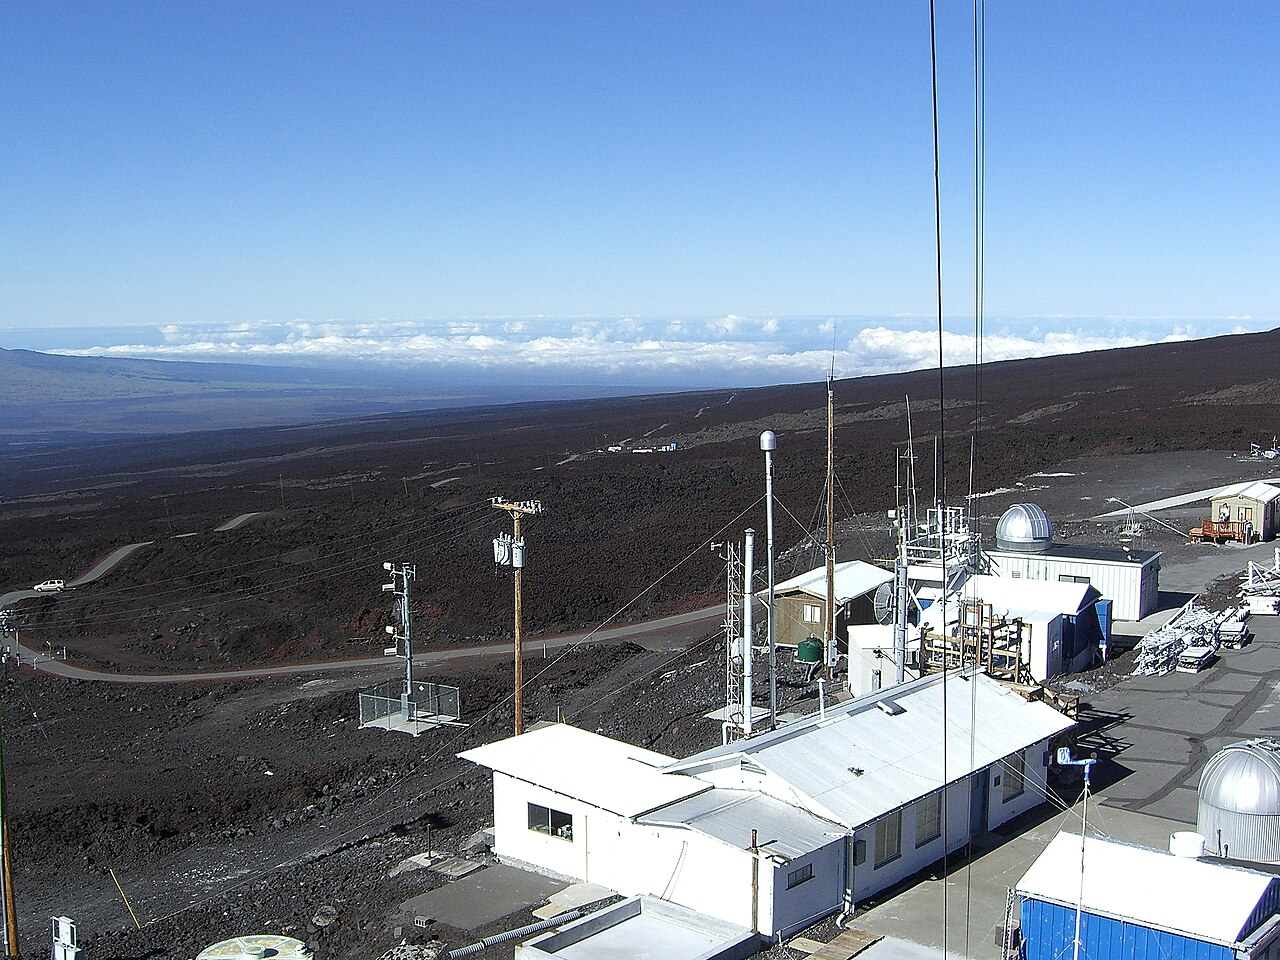
\includegraphics[width=0.56\linewidth]{images/book4/mauna-loa.jpg}\hspace{0.03\linewidth}
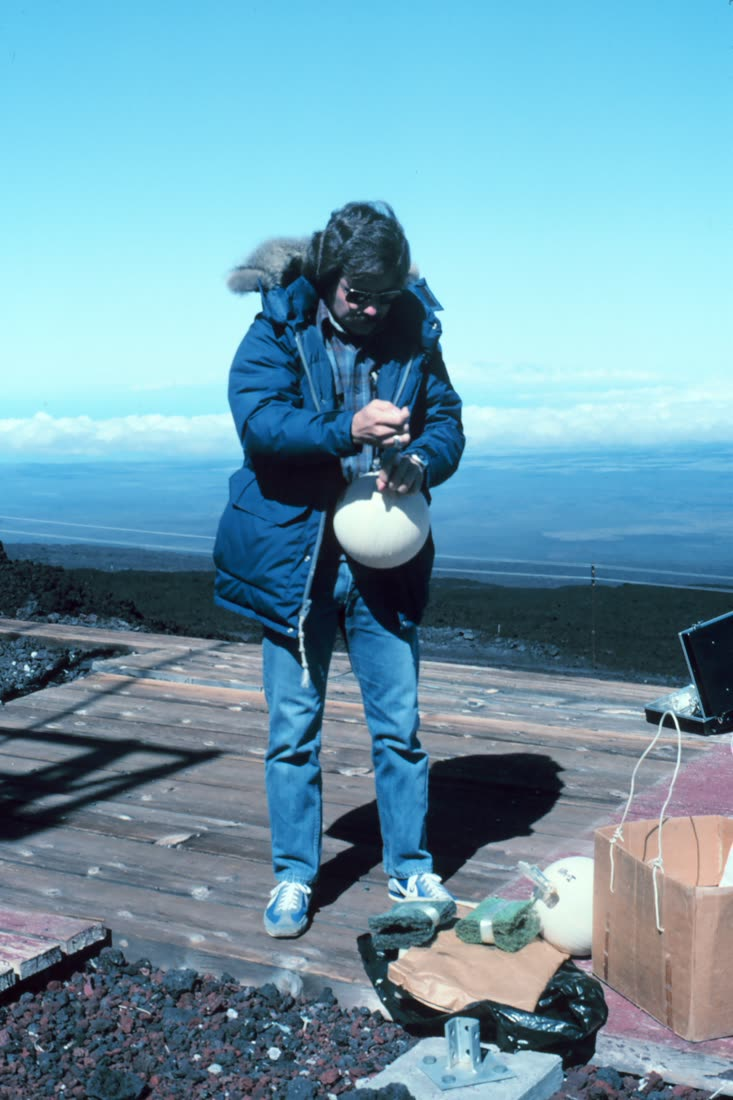
\includegraphics[width=0.33\linewidth]{images/book4/keeling-flask.jpg}

{\small Donde se dibuja la curva. Izquierda: el observatorio de la ladera
norte del Mauna Loa, a \qty{3400}{m} de altitud, por encima de la
inversión de los alisios que mantiene debajo el aire propio de la isla.
Derecha: toma de una muestra en un matraz en 1982; matraces como estos,
analizados en California, sirven para comprobar el analizador continuo y
se llenan en estaciones que van de Alaska al Polo Sur.}
\end{omfigure}

\section{El ciclo del nitrógeno}

\begin{proposition}[El ciclo del nitrógeno]\label{prop:b2:biogeochemical-cycles:nitrogen}
\index{ciclo del nitrógeno}\index{fijación del nitrógeno}\index{nitrificación}\index{desnitrificación}\index{proceso Haber--Bosch}\index{anammox}
El nitrógeno es abundante --- el aire contiene $4\times 10^{9}$~Tg de
$\mathrm{N_2}$ --- y escaso, porque el triple enlace del $\mathrm{N_2}$ solo lo
abren dos procesos: los rayos (unos pocos Tg al año) y la
\emph{fijación biológica del nitrógeno} por \omterm{def:b2:unicellular-diversity:prokaryote}{procariotas} dotados de
nitrogenasa, unos 100 Tg al año en tierra y 100 en el mar, con un coste
de 16 ATP por $\mathrm{N_2}$. El nitrógeno fijado recorre después una
escalera redox impulsada por microorganismos
(\cref{ch:b2:microbial-metabolism}): la \emph{amonificación} de la
materia muerta a $\mathrm{NH_4^{+}}$; la
\emph{nitrificación} del $\mathrm{NH_4^{+}}$ a $\mathrm{NO_2^{-}}$ y $\mathrm{NO_3^{-}}$ por
\omterm{def:b2:microbial-metabolism:trophic}{quimiolitótrofos} aerobios; la absorción de $\mathrm{NH_4^{+}}$ o de $\mathrm{NO_3^{-}}$ por
las plantas y su reducción de nuevo a amina; y, donde falta el oxígeno, la
\emph{\omterm{def:b2:microbial-metabolism:anaerobic}{desnitrificación}} del $\mathrm{NO_3^{-}}$ a $\mathrm{N_2}$ (con fugas de $\mathrm{N_2O}$)
y el \emph{anammox}, la oxidación anaerobia del amonio por el
nitrito hasta $\mathrm{N_2}$, que juntos devuelven al aire aproximadamente
tanto como toma la fijación. El \omterm{def:b2:biogeochemical-cycles:reservoir}{tiempo de residencia} de un átomo de
nitrógeno en la biosfera es de unos pocos cientos de años; en la
atmósfera, $4\times
10^{9}/400 \approx 10^{7}$ años. Desde 1913, el proceso
\emph{Haber--Bosch} fija nitrógeno industrialmente, hoy unos 120 Tg al
año, y las leguminosas cultivadas y la combustión de combustibles fósiles
añaden 60 y 30: la actividad humana fija tanto nitrógeno como todos los
procesos naturales juntos, y alimenta a la mitad de las personas vivas.
\end{proposition}

\begin{omfigure}
\begin{tikzpicture}[every node/.style={font=\scriptsize}, >=stealth, box/.style={draw, rounded corners, minimum width=1.9cm, minimum height=0.8cm, align=center, fill=#1}]
  \node[box=omDef!15] (n2) at (0,3.4) {$\mathrm{N_2}$ del aire\\$4\times 10^{9}$ Tg};
  \node[box=omThm!15] (org) at (-4.6,1.0) {N orgánico\\plantas, suelos, mar};
  \node[box=omProp!15] (nh4) at (-2.2,-0.8) {$\mathrm{NH_4^{+}}$};
  \node[box=omProp!15] (no2) at (2.2,-0.8) {$\mathrm{NO_2^{-}}$};
  \node[box=omProp!15] (no3) at (4.6,1.0) {$\mathrm{NO_3^{-}}$};
  \draw[->, thick] (n2) -- node[above left, align=right] {fijación\\nitrogenasa, 200\\Haber--Bosch 120} (org);
  \draw[->, thick] (org.south) -- node[below left] {amonificación} (nh4.north);
  \draw[->, thick] (nh4) -- node[below] {nitrificación} (no2);
  \draw[->, thick] (no2) -- node[below right] {nitrificación} (no3);
  \draw[->, thick] (no3) to[bend left=18] node[above, pos=0.72] {asimilación} (org);
  \draw[->, thick, omExo!80!black] (no3) -- node[above right, align=left] {desnitrificación\\(anóxica), fuga de $\mathrm{N_2O}$} (n2);
  \draw[->, thick, omExo!80!black] (no2) -- node[right, pos=0.55, align=left] {anammox\\(con $\mathrm{NH_4^{+}}$)} (n2);
  \node[anchor=north, align=center] at (0,-1.5) {flujos en Tg de N por año; todas las etapas salvo la asimilación y la amonificación las realizan procariotas};
\end{tikzpicture}

{\small El \omterm{prop:b2:biogeochemical-cycles:nitrogen}{ciclo del nitrógeno} como escalera redox (las plantas asimilan
tanto el amonio como el nitrato). La fijación y la \omterm{def:b2:microbial-metabolism:anaerobic}{desnitrificación}, las
dos puertas hacia la atmósfera, son ambas microbianas; la puerta
industrial iguala hoy a la natural.}
\end{omfigure}

\begin{proof}[Evidencia]
El bosque experimental de Hubbard Brook, Nuevo Hampshire: en 1965 se taló a
matarrasa una cuenca entera, que se mantuvo desnuda con herbicida, mientras
que una cuenca vecina se dejó intacta, y durante años se aforaron y
analizaron los arroyos que drenaban cada una. La cuenca desnuda perdía
nitrato a un ritmo sesenta veces superior al de la cuenca de control ---
todo el capital de nitrógeno del suelo, que las plantas ya no absorbían,
se nitrificaba y era arrastrado, llevándose consigo calcio y potasio y
acidificando el arroyo. El experimento mostró lo cerrado que es el ciclo
en un bosque intacto (unos pocos kilogramos de nitrógeno perdidos por
hectárea y por año, frente a cientos reciclados) y lo que lo rompe.
\end{proof}

\section{El fósforo y el azufre}

\begin{proposition}[Dos ciclos sin un gas rápido]\label{prop:b2:biogeochemical-cycles:ps}
\index{ciclo del fósforo}\index{ciclo del azufre}\index{eutrofización}\index{dimetilsulfuro}
El \emph{fósforo} no tiene forma gaseosa. Entra en los ecosistemas por la
meteorización del apatito de las rocas, unos 20 Tg al año sobre toda la
superficie terrestre, se recicla muchas veces dentro de los suelos y los
lagos --- un ion fosfato de las aguas superficiales de un lago se absorbe
en unas horas --- y sale hacia los sedimentos, donde permanece durante
los $10^{8}$ años de un ciclo de las rocas. La vida es, por tanto,
ahorradora de fósforo y está limitada por el fósforo: el \omterm{def:b2:biogeochemical-cycles:reservoir}{tiempo de
residencia} en el océano es de unos \num{20000} años, y el fosfato del
océano profundo, que los afloramientos suben a la superficie, fija su
productividad. La minería lleva hoy a las tierras de cultivo
aproximadamente tanto fósforo como libera la meteorización, y su
escorrentía hacia los lagos causa la \emph{eutrofización}: una
proliferación de algas, su descomposición, el consumo del oxígeno y la
muerte de los peces --- los experimentos de Schindler en lagos enteros de
Ontario en la década de 1970, con una mitad de un lago fertilizada con
fósforo y la otra no, mostraron que el fósforo solo bastaba para
desencadenarla, y llevaron a retirarlo de los detergentes. El
\emph{azufre} tiene a la vez un ciclo de las rocas (yeso, pirita) y una
fase gaseosa: el $\mathrm{SO_2}$ de los volcanes y del carbón, el $\mathrm{H_2S}$ de los
sedimentos anóxicos y el \emph{dimetilsulfuro} del plancton marino, cuyos
productos de oxidación siembran las nubes sobre el océano. La combustión
del carbón triplicó el \omterm{def:b2:biogeochemical-cycles:reservoir}{flujo} de azufre hacia el aire en el siglo XX y dio
a Europa y a Norteamérica su lluvia ácida; los depuradores de gases la
invirtieron en unas décadas, puesto que el \omterm{def:b2:biogeochemical-cycles:reservoir}{tiempo de residencia} del ciclo
en el aire es de unos pocos días.
\end{proposition}

\begin{omfigure}
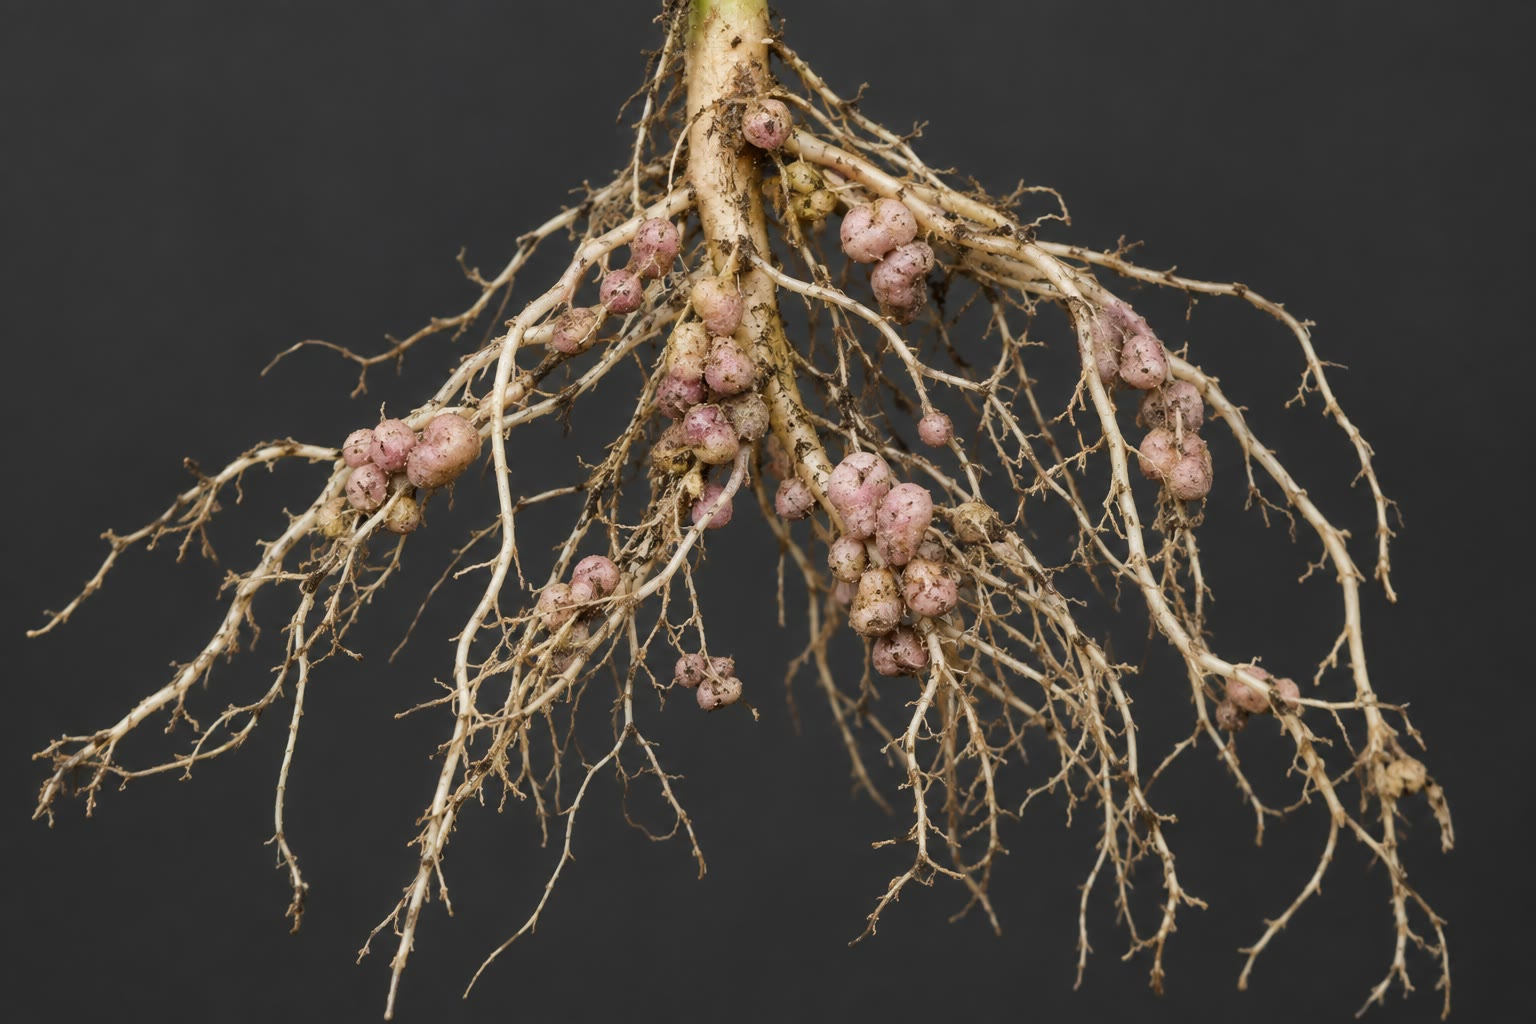
\includegraphics[width=0.44\linewidth]{images/book4/ai/b4-25-root-nodules.jpg}\hspace{0.04\linewidth}
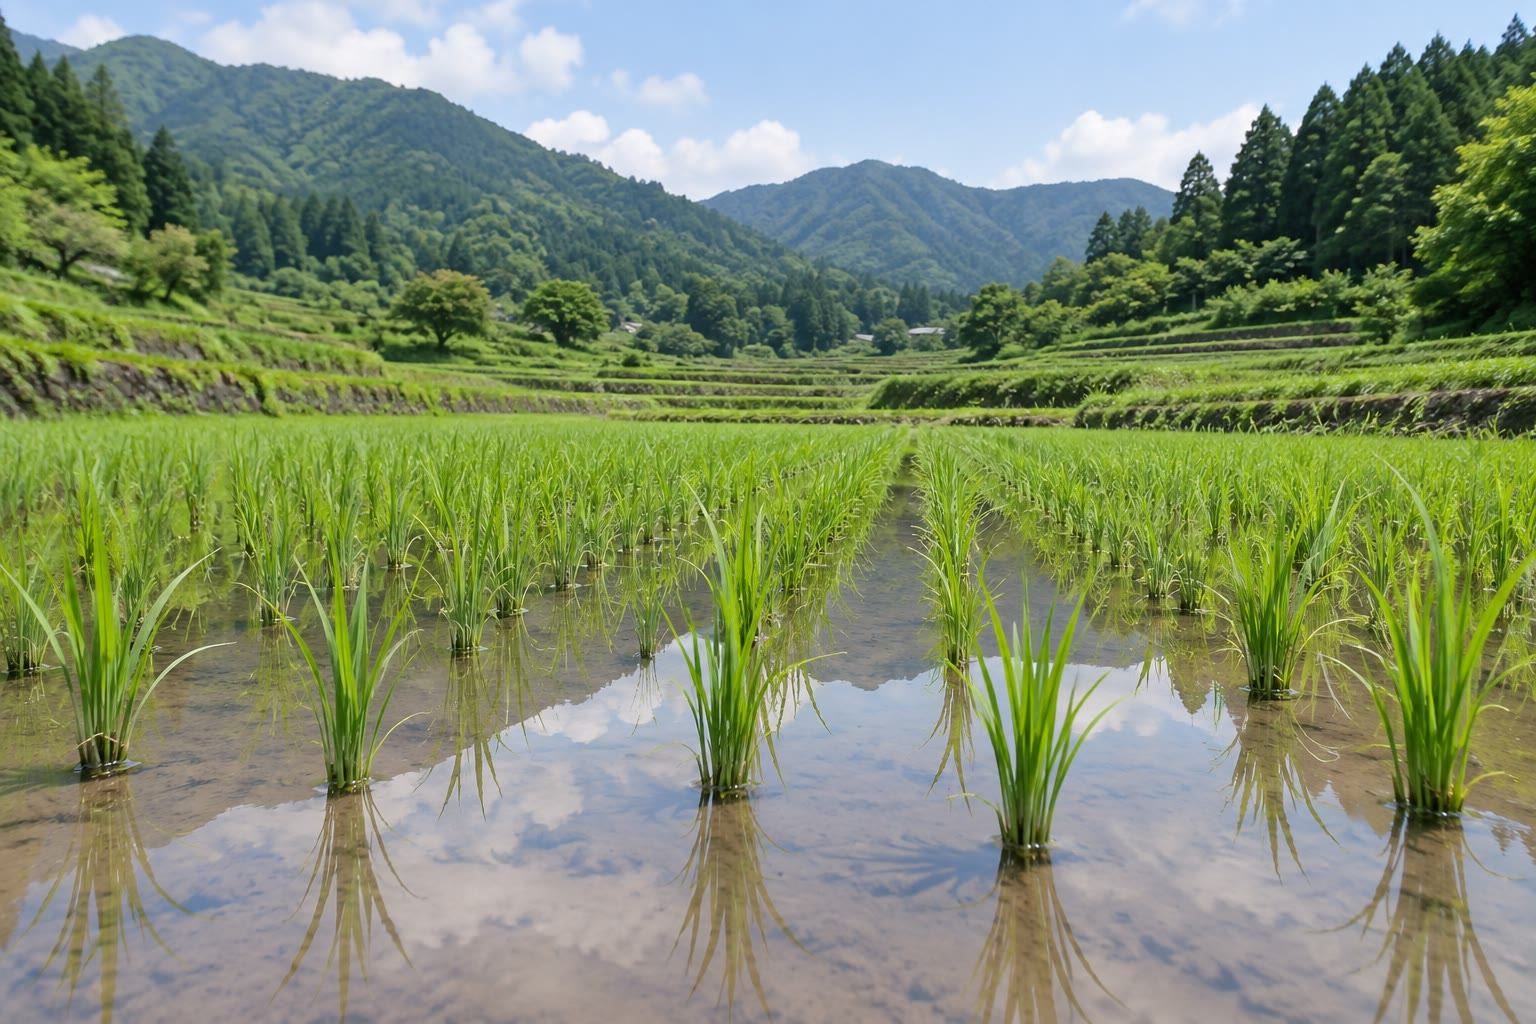
\includegraphics[width=0.44\linewidth]{images/book4/ai/b4-25-rice-paddy.jpg}

{\small Dos puertas del \omterm{prop:b2:biogeochemical-cycles:nitrogen}{ciclo del nitrógeno}. Izquierda: nódulos radicales
de una leguminosa, cada uno una cámara en la que los rizobios fijan
nitrógeno para su hospedador. Derecha: un arrozal inundado, anóxico bajo
la superficie, donde la \omterm{def:b2:microbial-metabolism:anaerobic}{desnitrificación} devuelve nitrógeno al aire y los
metanógenos producen metano.}
\end{omfigure}

\section{El planeta perturbado}

\begin{example}[Lo que dicen las cifras]\label{ex:b2:biogeochemical-cycles:numbers}
Unas emisiones de \qty{10}{GtC} al año con una \omterm{prop:b2:biogeochemical-cycles:carbon}{fracción atmosférica} de
$0.45$ dejan \qty{4.5}{GtC}, o \qty{2.1}{ppm}, en el aire cada año
--- la pendiente observada. Las emisiones acumuladas desde 1850 son de
unas \qty{700}{GtC}, de las que \qty{290}{GtC} están en el aire (140~ppm)
y el resto en el océano y en las tierras emergidas. Para mantener la
atmósfera en cualquier nivel, las emisiones netas deben caer hasta lo que
pueden absorber los sumideros lentos --- la mezcla con el océano profundo y
la meteorización, que juntas no llegan a \qty{1}{GtC} al año:
las \emph{emisiones netas nulas} no son un eslogan, sino la condición de
\omterm{def:b2:biogeochemical-cycles:reservoir}{estado estacionario} del \omterm{thm:b2:biogeochemical-cycles:box}{modelo de caja} con un $\tau$ muy largo. En el caso
del nitrógeno, la duplicación del \omterm{def:b2:biogeochemical-cycles:reservoir}{flujo} de nitrógeno fijado ha duplicado
el nitrato de los ríos, ha producido zonas muertas en la desembocadura
del Misisipi y en el Báltico, y ha elevado en una quinta parte el
$\mathrm{N_2O}$ de la atmósfera, un gas de efecto invernadero con un \omterm{def:b2:biogeochemical-cycles:reservoir}{tiempo de
residencia} de un siglo. El \cref{ch:b2:global-change} sigue las
consecuencias para los seres vivos.
\end{example}

\section{Ejercicios}

\begin{exercise}[$\star$]\label{exo:b2:biogeochemical-cycles:1}
Defínanse \omterm{def:b2:biogeochemical-cycles:reservoir}{reservorio}, \omterm{def:b2:biogeochemical-cycles:reservoir}{flujo} y \omterm{def:b2:biogeochemical-cycles:reservoir}{tiempo de residencia}, y calcúlese el \omterm{def:b2:biogeochemical-cycles:reservoir}{tiempo
de residencia} del carbono en las plantas terrestres (450 GtC,
fotosíntesis de 120 GtC al año) y en el océano profundo (\num{37000} GtC,
intercambio de unas 100 GtC al año).
\end{exercise}

\begin{exercise}[$\star$]\label{exo:b2:biogeochemical-cycles:2}
Conviértanse \qty{2.5}{ppm} al año en GtC, y \qty{10}{GtC} de emisiones
en ppm.
\end{exercise}

\begin{exercise}[$\star$]\label{exo:b2:biogeochemical-cycles:3}
Nómbrense los dos procesos naturales que abren el $\mathrm{N_2}$, el proceso
que lo devuelve y las tres etapas redox intermedias, con los organismos
responsables.
\end{exercise}

\begin{exercise}[$\star$]\label{exo:b2:biogeochemical-cycles:4}
¿Por qué el fósforo limita la productividad con más frecuencia que el
nitrógeno a escala geológica, y el nitrógeno con más frecuencia que el
fósforo en una estación dada?
\end{exercise}

\begin{exercise}[$\star\star$]\label{exo:b2:biogeochemical-cycles:5}
Un lago de \qty{e7}{m^3} recibe \qty{2}{t} de fósforo al año y renueva el
\qty{20}{\%} de su agua anualmente. Calcúlense su concentración de fósforo
en \omterm{def:b2:biogeochemical-cycles:reservoir}{estado estacionario} y el tiempo necesario para alcanzar el \qty{90}{\%}
de ella desde que empieza el aporte. ¿Y si el aporte se reduce a la mitad?
\end{exercise}

\begin{exercise}[$\star\star$]\label{exo:b2:biogeochemical-cycles:6}
A partir de los datos de Keeling, calcúlese la tasa media de crecimiento
del $\mathrm{CO_2}$ en la década de 1960 (de 316 a \qty{325}{ppm} en diez años) y en
la de 2010 (de 390 a 411 en nueve años), en ppm al año y en GtC al año.
\end{exercise}

\begin{exercise}[$\star\star$]\label{exo:b2:biogeochemical-cycles:7}
Los dientes de sierra estacionales del Mauna Loa tienen una amplitud de
unas \qty{6}{ppm} de pico a valle. Conviértase en GtC y compárese con la
producción primaria neta anual de las tierras del hemisferio norte, unas
\qty{35}{GtC}. ¿Por qué son tan pequeños los dientes de sierra?
\end{exercise}

\begin{exercise}[$\star\star$]\label{exo:b2:biogeochemical-cycles:8}
La nitrogenasa gasta 16 ATP por $\mathrm{N_2}$. Para una leguminosa que fija
\qty{200}{kg} de nitrógeno por hectárea y por año, calcúlense los moles de
$\mathrm{N_2}$ fijados y el ATP gastado, y la masa de glucosa que representa
ese ATP (unos 30 ATP por glucosa). ¿Qué fracción de los fotosintatos de un
cultivo de \qty{10}{t/ha} supone?
\end{exercise}

\begin{exercise}[$\star\star$]\label{exo:b2:biogeochemical-cycles:9}
El plancton crece con el cociente de Redfield $\mathrm{C:N:P} = 106:16:1$.
El agua de mar profunda contiene \qty{2.2}{\micro mol/kg} de fosfato y
\qty{32}{\micro mol/kg} de nitrato. ¿Cuál se agota primero cuando una masa
de agua sube a la superficie, y cuánto carbono se fija antes de que ocurra?
\end{exercise}

\begin{exercise}[$\star\star\star$]\label{exo:b2:biogeochemical-cycles:10}
Trátese la atmósfera como una caja con un exceso de carbono $E$ que los
sumideros retiran a una velocidad $E/\tau$ y que alimentan unas emisiones
$Q$. Con $\tau =
50$ años y $Q = \qty{10}{GtC/yr}$, ¿cuál es el exceso en \omterm{def:b2:biogeochemical-cycles:reservoir}{estado
estacionario} y a cuántas ppm corresponde? Explíquese por qué la respuesta
real es peor.
\end{exercise}

\begin{exercise}[$\star\star\star$]\label{exo:b2:biogeochemical-cycles:11}
Los ensayos nucleares duplicaron el $\mathrm{{}^{14}C}$ de la atmósfera en 1963;
después, el exceso se redujo a la mitad aproximadamente cada 11 años,
aunque el $\mathrm{{}^{14}C}$
tiene un periodo de semidesintegración de 5730 años. Explíquese qué se
midió y qué dicen esos 11 años sobre el \omterm{prop:b2:biogeochemical-cycles:carbon}{ciclo del carbono}.
\end{exercise}

\begin{exercise}[$\star\star\star$]\label{exo:b2:biogeochemical-cycles:12}
``La humanidad ha duplicado el \omterm{prop:b2:biogeochemical-cycles:nitrogen}{ciclo del nitrógeno} y apenas ha rozado el
\omterm{prop:b2:biogeochemical-cycles:carbon}{ciclo del carbono}.'' Discútase con cifras: \omterm{def:b2:biogeochemical-cycles:reservoir}{flujos} fijados, fracciones del
\omterm{def:b2:biogeochemical-cycles:reservoir}{flujo} natural y \omterm{def:b2:biogeochemical-cycles:reservoir}{reservorios} afectados.
\end{exercise}

\section{Problema: el balance de carbono de un siglo}

\begin{problem}[{Problema de fin de semana --- un siglo de emisiones pasado
por el modelo de caja de la atmósfera, la parte del océano y la de las
tierras emergidas, la cascada del nitrógeno desde un campo fertilizado
hasta una zona muerta y el balance de fósforo de un lago, hasta llegar a
la fracción atmosférica, la concentración atmosférica en 2100 y el
nitrógeno perdido por hectárea}]
\label{pb:b2:biogeochemical-cycles:1}
Datos. Atmósfera en 1850: \qty{285}{ppm}; \qty{1}{ppm} $=
\qty{2.13}{GtC}$. Emisiones acumuladas 1850--2020: \qty{700}{GtC};
$\mathrm{CO_2}$ atmosférico en 2020: \qty{412}{ppm}. Un campo de
\qty{1}{ha} recibe \qty{150}{kg} de abono nitrogenado al año; el cultivo
absorbe el \qty{60}{\%}, el \qty{25}{\%} se desnitrifica y el resto se
lixivia. Un lago de \qty{5e7}{m^3} renueva una décima parte de su agua al
año y recibe \qty{5}{t} de fósforo al año.

\medskip
\noindent\textbf{Parte I --- La \omterm{prop:b2:biogeochemical-cycles:carbon}{fracción atmosférica}.}
\begin{enumerate}
  \item Calcúlense el carbono atmosférico en 1850 y en 2020, y el aumento
        en GtC.
  \item Calcúlese la \omterm{prop:b2:biogeochemical-cycles:carbon}{fracción atmosférica} durante 1850--2020.
  \item ¿Dónde está el resto? Dense los dos sumideros y, a partir de la
        proposición, sus partes aproximadas.
  \item Si el océano ha absorbido el \qty{25}{\%} de las emisiones, ¿en
        qué proporción ha aumentado su carbono inorgánico disuelto,
        \qty{38000}{GtC}? ¿Por qué, aun así, el océano superficial se
        acidifica de forma medible?
  \item ¿Por qué la \omterm{prop:b2:biogeochemical-cycles:carbon}{fracción atmosférica} se mantiene aproximadamente
        constante mientras las emisiones crecen de forma exponencial?
        (Considérese el \omterm{thm:b2:biogeochemical-cycles:box}{modelo de caja} con
        $Q \propto e^{t/T}$ y un sumidero $E/\tau$.)
  \item ¿En qué se convertiría la \omterm{prop:b2:biogeochemical-cycles:carbon}{fracción atmosférica} si las emisiones se
        mantuvieran constantes durante muchos siglos?
\end{enumerate}

\medskip
\noindent\textbf{Parte II --- El siglo que viene.}
Modelícese el exceso de carbono $E$ (por encima del nivel de 1850) con
$\mathrm{d}E/\mathrm{d}t = Q - E/\tau$, $\tau = 100$ años.
\begin{enumerate}[resume]
  \item Calcúlese el exceso en 2020 en GtC.
  \item Con $Q$ mantenida en \qty{10}{GtC/yr}, calcúlense el exceso en
        \omterm{def:b2:biogeochemical-cycles:reservoir}{estado estacionario} y la concentración que implica.
  \item Resuélvase $E(t)$ a partir de 2020 con $Q = 10$ y dense $E$ en
        2100 y la concentración.
  \item Ahora $Q$ baja linealmente hasta cero entre 2020 y 2070 y se
        mantiene en cero. Calcúlese $E$ en 2070 (intégrese la ecuación; la
        solución particular para una $Q$ lineal es lineal más una
        constante) y en 2100.
  \item Compárense las dos concentraciones en 2100.
  \item ¿Por qué un único $\tau$ es optimista para el segundo escenario?
\end{enumerate}

\medskip
\noindent\textbf{Parte III --- La cascada del nitrógeno.}
\begin{enumerate}[resume]
  \item Calcúlense el nitrógeno absorbido por el cultivo, el desnitrificado
        y el lixiviado, por hectárea y por año.
  \item El nitrógeno lixiviado llega a un río en forma de nitrato y
        después al mar, donde el plancton lo utiliza según el cociente de
        Redfield. ¿Cuánto carbono permite fijar al plancton?
  \item Ese carbono se hunde y se respira en profundidad, consumiendo
        oxígeno a razón de 1 $\mathrm{O_2}$ por C. Calcúlese el oxígeno
        consumido, en moles y en kilogramos.
  \item Un metro cúbico de agua de mar contiene unos \qty{0.25}{mol} de
        $\mathrm{O_2}$ cuando está saturado. ¿Cuántos metros cúbicos de
        agua de fondo desoxigena la lixiviación de una hectárea?
  \item La fracción desnitrificada escapa en parte como $\mathrm{N_2O}$,
        el \qty{1}{\%} del nitrógeno desnitrificado. Calcúlense el $\mathrm{N_2O}$
        por hectárea y por año, y su equivalente de calentamiento en $\mathrm{CO_2}$
        (el $\mathrm{N_2O}$ equivale a 270 veces el $\mathrm{CO_2}$ por kilogramo).
  \item Compárese con el $\mathrm{CO_2}$ emitido para fabricar el abono
        (unos \qty{4}{kg} de $\mathrm{CO_2}$ por kilogramo de nitrógeno por
        el \omterm{prop:b2:biogeochemical-cycles:nitrogen}{proceso Haber--Bosch}).
\end{enumerate}

\medskip
\noindent\textbf{Parte IV --- El lago.}
\begin{enumerate}[resume]
  \item Calcúlense el \omterm{def:b2:biogeochemical-cycles:reservoir}{tiempo de residencia} del fósforo en el lago si la
        única pérdida es la renovación del agua, y su concentración en
        \omterm{def:b2:biogeochemical-cycles:reservoir}{estado estacionario} en \unit{mg/m^3}.
  \item Los lagos con más de \qty{30}{mg/m^3} de fósforo son eutróficos.
        ¿Lo es este?
  \item La sedimentación retira fósforo con su propia constante de tiempo
        de 5 años. Vuélvanse a calcular el \omterm{def:b2:biogeochemical-cycles:reservoir}{tiempo de residencia} y la
        concentración.
  \item El aporte se reduce a \qty{1}{t} al año. Calcúlense el nuevo
        \omterm{def:b2:biogeochemical-cycles:reservoir}{estado estacionario} y el tiempo necesario para quedar a menos del
        \qty{10}{\%} de él.
  \item ¿Por qué muchos lagos se recuperan más despacio de lo que predice
        este cálculo?
  \item Calcúlese el carbono que el fósforo del lago puede incorporar al
        plancton cada año según el cociente de Redfield, a partir del
        aporte de \qty{5}{t}.
  \item Enúnciese el resultado: la \omterm{prop:b2:biogeochemical-cycles:carbon}{fracción atmosférica}, las dos
        concentraciones en 2100 y el nitrógeno lixiviado por hectárea.
\end{enumerate}
\end{problem}
